\section{Evaluation}
\label{sec:eval}

We ask four questions.
\begin{itemize}
  \item[\rqref{1}] Does the typed grammar reach more of \pg than a
    random-mutation generator in the same time: more valid statements, more
    covered lines and branches, more SQL features and plan shapes?
  \item[\rqref{2}] Which bugs does \tool find, and how precise is each oracle?
  \item[\rqref{3}] On real bugs put back into \pg, which configuration finds
    how many, and how fast?
  \item[\rqref{4}] What does the commit-directed LLM extension add, and what
    does it cost in tokens, money and repair rounds?
\end{itemize}

\subsection{Subject and Benchmark}
\label{sec:subjects}

All servers are built from \pg master \texttt{26bd08fb} (16~October~2026) with
assertions on. For \rqref{3} we built a benchmark in the style of
Magma~\cite{hazimeh2020magma} by reverting fixes: every commit between
31~July and 16~October~2026 that fixes a bug in the optimiser, executor,
parser, rewriter or a SQL-callable function, adds a regression test, and
reverts cleanly alone and together with the others, 23 in all. We build the
\emph{fixed} server, one \emph{solo} server per bug (only that fix reverted),
and the \emph{injected} server (all 23 reverted) on which the campaigns run.
A proof of concept (PoC) written from each regression test changes its result
for 20 bugs: 8 wrong results, 5 internal errors, 4 assertion failures, 2
missing errors and 1 wrong error. A crash-only fuzzer can see only the 9
assertions and internal errors. The other three change only the plan, or need an
equality operator that returns NULL for non-NULL inputs, and leave the
denominator. On the injected server every PoC shows the symptom of its solo
server.

\subsection{Configurations}
\label{sec:baselines}

The configurations (\emph{arms}) share server, schema, executor, oracles,
budget and per-trial seeds and differ only in the generator. \arm{Random}
mutates seed queries at the token level and attaches no metamorphic checks.
\arm{Grammar} is Step 1 alone. \arm{Grammar+Oracles} adds Steps 2--4: metamorphic
checks (including RLS and CERT) on half the queries, plan-shape guidance,
feedback weights and data-profile literals; \arm{Grammar+Oracles, flat} is the
same without the weights. \arm{+LLM} adds the fragments, seeds and rewrites that
passed the \gate, and \arm{+LLM fragments} and \arm{+LLM seeds} use one of
them. The commit miner excludes the 23 benchmark fixes. All arms use the
plan-variant oracle and, in \rqref{3}, the cross-version oracle.

\subsection{Setup}
\label{sec:setup}
\tool is about 10{,}500 lines of Python with 151 unit tests; it drives \pg
through \texttt{psycopg} and reads the server log for assertion and crash
evidence. Each arm runs 5 one-hour trials with four workers, one server each.
\rqref{1}, \rqref{2} and \rqref{4} ran on one laptop (WSL2, 24 logical cores),
\rqref{3} on another, so each experiment is compared on one machine.
The cross-version reference is \pg 18.6. Following
Klees et al.~\cite{klees2018evaluating}, and Arcuri and
Briand~\cite{arcuri2011practical}, we report medians, compare arms with the
two-sided Mann--Whitney U test, and give the Vargha--Delaney
$\hat{A}_{12}$ effect size~\cite{vargha2000a12}. With 5 trials per arm the
smallest possible two-sided $p$ is 0.008, so we read effect sizes, not only
$p$. Coverage is sampled every 300 seconds per worker, so the first point of every curve is the server's start-up coverage.

\paragraph{The language model.} In the client's manual mode a script answered
the prompts with Google Gemini Flash models on the free tier (9 answers by
\texttt{gemini-3.6-flash}, 2 by \texttt{gemini-3.8-flash}, 14 by
\texttt{gemini-3-flash-preview}); the daily quota limited \rqref{4} to 10 of the
25 mined commits. The results of \rqref{4} hold for these models.

\subsection{\rqref{1}: Reach}
\label{sec:rq1}

Table~\ref{tab:rq1} gives the medians of the seven arms and
Figure~\ref{fig:rq1} the growth over time.

\begin{table*}[t]
  \centering
  \small
  \caption{\rqref{1}: median of 5 one-hour trials per arm on an instrumented
  \pg master. Valid is the share of statements that run without error; lines
  and branches are of the backend (gcov); features are of a catalogue of 148.}
  \label{tab:rq1}
  \begin{tabular}{lrrrrrr}
    \toprule
    Arm & Valid (\%) & Lines (\%) & Branches (\%) & Features & Plan shapes & Test cases \\
    \midrule
    \arm{Random} & 26.0 & 22.2 & 15.1 & 23 & 43 & 1{,}074{,}240 \\
    \arm{Grammar} & 99.3 & 36.7 & 27.1 & 101 & 20{,}279 & 71{,}228 \\
    \arm{Grammar+Oracles} & 96.3 & 36.2 & 26.7 & 101 & 34{,}313 & 58{,}601 \\
    \arm{Grammar+Oracles, flat} & 99.4 & 36.2 & 26.8 & 101 & 23{,}997 & 64{,}923 \\
    \arm{+LLM fragments} & 95.5 & 35.7 & 26.5 & 104 & 25{,}972 & 48{,}222 \\
    \arm{+LLM seeds} & 98.3 & 35.6 & 26.4 & 106 & 29{,}274 & 63{,}655 \\
    \arm{+LLM (both)} & 95.3 & 35.7 & 26.4 & 106 & 26{,}375 & 46{,}754 \\
    \bottomrule
  \end{tabular}

\end{table*}

\begin{figure}[t]
  \centering
  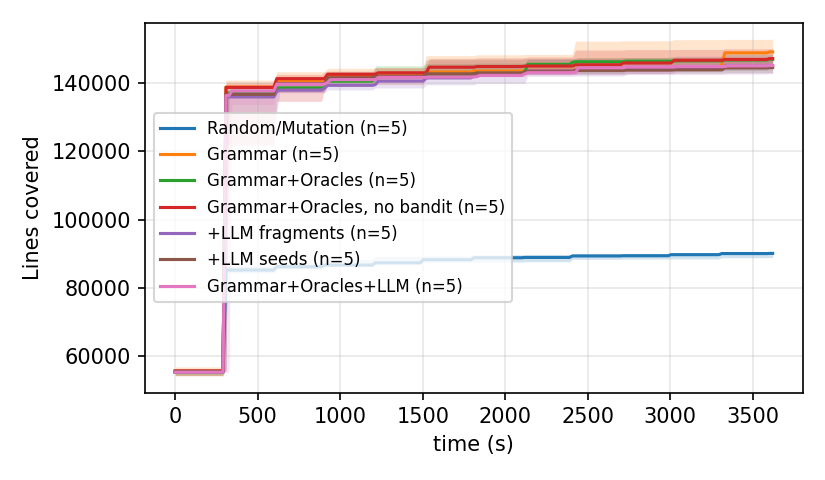
\includegraphics[width=0.44\linewidth]{figures/rq1_lines}
  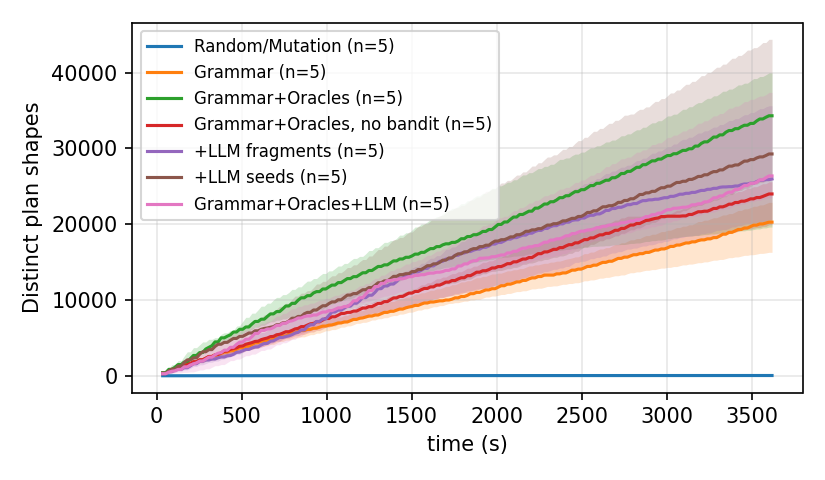
\includegraphics[width=0.44\linewidth]{figures/rq1_plans}
  \caption{\rqref{1}: lines covered (left) and distinct plan shapes (right) over
  time, median and interquartile band of 5 trials per arm.}
  \label{fig:rq1}
\end{figure}

\begin{observation}
\label{obs:grammar}
The typed grammar reaches far more than random mutation: 36.7\% against 22.2\%
of lines ($\hat{A}_{12}=1.00$, $p=0.008$), 101 against 23 SQL features, and
99.3\% against 26.0\% valid statements, although the random arm runs 15 times
more test cases.
\end{observation}

\begin{observation}
\label{obs:oracles-reach}
The oracles do not add line coverage (36.7\% to 36.2\%, $p=0.42$) but they
roughly double the plan shapes (20{,}279 to 34{,}313, $\hat{A}_{12}=0.84$,
$p=0.095$, so with 5 trials this is an effect size, not a significant
difference). The feedback weights contribute: without them the same arm
reaches 23{,}997 plan shapes ($\hat{A}_{12}=0.80$, $p=0.15$), at the price of
validity (96.3\% against 99.4\%, $p=0.016$).
\end{observation}

Oracles also cost throughput: the plan-variant runs and metamorphic checks
lower the statements per second from 67 to 40.

\subsection{\rqref{2}: Bugs and Oracle Precision}
\label{sec:rq2}

Across the \rqref{1} and \rqref{3} campaigns, plus the earlier hunt and smoke
runs, \tool reported 93 distinct bug candidates (after de-duplication by
signature). We triaged all of them (Section~\ref{sec:triage}) and
Table~\ref{tab:rq2} gives the verdicts per oracle.

\begin{table*}[t]
  \centering
  \small
  \caption{\rqref{2}: verdict of every triaged candidate per oracle. Duplicate:
  a real bug that had already been reported upstream. False positives include
  one intended change between versions. Flaky: did not reproduce in three
  re-runs. Open: not decided yet.}
  \label{tab:rq2}
  \begin{tabular}{lrrrrrr}
    \toprule
    Oracle & Candidates & Real & Duplicate & False pos. & Flaky & Open \\
    \midrule
    assertion & 15 & 3 & 10 & 1 & 1 & 0 \\
    crash & 1 & 0 & 0 & 1 & 0 & 0 \\
    cross-version & 25 & 0 & 0 & 7 & 18 & 0 \\
    internal\_error & 4 & 2 & 1 & 0 & 1 & 0 \\
    mm: expr & 3 & 1 & 1 & 1 & 0 & 0 \\
    mm: rls & 5 & 0 & 0 & 5 & 0 & 0 \\
    mm: tlp\_having & 4 & 0 & 0 & 4 & 0 & 0 \\
    mm: tlp\_where & 4 & 1 & 1 & 2 & 0 & 0 \\
    plan-variant & 32 & 1 & 2 & 21 & 8 & 0 \\
    \midrule
    all & 93 & 8 & 15 & 42 & 28 & 0 \\
    \bottomrule
  \end{tabular}

\end{table*}

\paragraph{Bugs.} Table~\ref{tab:bugs} lists the ten bugs we reported. Six
came from running the fuzzer (the campaigns and later runs on newer master builds); four came from
the targeted bug hunt that accompanied them, in which we audited recent planner and executor features with
differential probes. Eight of the ten bugs are fixed upstream, six of them with fixes written by the
authors. The other two are open with our patches. The oracles also found three bugs reported by others days
before us, which we count as duplicates: a wrong result of self-join
elimination under \texttt{ROLLUP} in 18.6 (\#19800, a plan variant), \#19772
(the \texttt{(SELECT e)} rewrite) and \#19784.

\begin{table*}[t]
  \centering
  \footnotesize
  \caption{The ten bugs we reported upstream, the oracle that recognises each,
  and their state on 13~November~2026. All reproduce on the base build
  \texttt{26bd08fb}, which predates the fixes.}
  \label{tab:bugs}
  \begin{tabular}{@{}llll@{}}
    \toprule
    Bug & Report & Oracle & State \\
    \midrule
    \texttt{JSON\_TABLE} assigns no collations & \#19768 & assertion & fixed (our patch) \\
    \texttt{range @> NULL} folded to a constant & \#19793 & \texttt{(SELECT e)} rewrite & reported, patch \\
    \texttt{MERGE}: SubPlan with no parent & \#19802 & internal error & fixed \\
    parallel \texttt{Append} assertion & \#19803 & TLP (\arm{+LLM fragments}) & fixed \\
    \texttt{to\_char(NaN)} breaks \texttt{NORMALIZE} & \#19771 & assertion & fixed (our patch) \\
    \texttt{NOT IN} anti-join ignores a cast & pgsql-bugs & TLP & fixed (our patch) \\
    \texttt{IGNORE NULLS} frame never returns & pgsql-bugs & hang & fixed (our patch) \\
    duplicate statistics expression & pgsql-bugs & assertion & fixed (our patch) \\
    non-finite imported MCV frequencies & pgsql-hackers & CERT estimate & patch \\
    \texttt{corr()} of a constant under partial aggregation & \#19826 & plan variant & fixed (our patch) \\
    \bottomrule
  \end{tabular}
\end{table*}

\paragraph{Rediscovery.} We added each reproducer as a seed that carries its own
check (for a wrong result, the query that must agree), extended the grammar with
what the four hunt bugs need (statistics on expressions, statistics import with
boundary values, a user-defined implicit cast, \texttt{IGNORE NULLS} over
whole-partition frames), and added a \emph{hang} oracle that restarts a server
whose statement outlives its \texttt{statement\_timeout} by ten seconds. One
150-second trial of \arm{Grammar+Oracles} on the base build then reported all
nine bugs reported up to that point, each matched to its catalogue entry, at unchanged validity (99.3\%).
With the tenth reproducer added (\#19826, found by the plan-variant oracle
under partitionwise aggregation), the one-command reproduction, one
150-second trial that replays the seeds in turn, reports all ten bugs.

\begin{observation}
\label{obs:wrong}
Plan-variant and metamorphic oracles found real wrong results in released
versions that no crash oracle can see (BUG~\#19793 and \#19800).
\end{observation}

\paragraph{Precision.} Of the 93 candidates, 28 (30\%) did not reproduce in
three re-runs. Of the 65 others, 8 are real, 15 are duplicates of real bugs and
42 are false positives, so the precision is $8/50=0.16$ without duplicates and
$23/65=0.35$ if duplicates count as true positives. The false positives come
from few classes: six were fixed before the campaigns, and five that the
campaigns revealed were fixed \emph{after} them, tested on the stored
reproducers but not re-measured.
They are equal \texttt{interval} values printed differently depending on
join order (16 candidates; the digest now uses \pg's interval equality),
order-sensitive aggregates sorted by a key that is not the value, such as
\texttt{ORDER BY NULL} (2), state that diverges in the cross-version oracle
after an \texttt{INSERT} only master accepts (5), an RLS rewrite that left a
protected table inside a repeated sub-select unfiltered (5), and an LLM rewrite
that is not an identity (Section~\ref{sec:rq4}). One remaining candidate is
a new bug, which we reported as BUG~\#19826: \texttt{corr()} of a constant input is NULL
serially but 1 under partial aggregation. It is fixed upstream with our patch
(\texttt{ef1b7404}, back-patched to 19).

\subsection{\rqref{3}: Re-injected Bugs}
\label{sec:rq3}

\begin{table*}[t]
  \centering
  \small
  \caption{\rqref{3}: trials (of 5) in which an arm found each re-injected bug,
  with the median time to the first finding. The rows below list, per symptom,
  how many bugs an arm found at all. Only bugs found by some arm have their own
  row; 18 of 20 were found by none.}
  \label{tab:rq3}
  \begin{tabular}{llrrrr}
    \toprule
    Bug & Symptom & \arm{Random} & \arm{Grammar} & \arm{Grammar+Oracles} & \arm{+LLM (both)} \\
    \midrule
    \texttt{11b56ee2} & assertion & 0/5 & 0/5 & 1/5 (2901\,s) & 1/5 (1858\,s) \\
    \texttt{dfcf6fa7} & internal error & 0/5 & 5/5 (458\,s) & 4/5 (509\,s) & 5/5 (1109\,s) \\
    \midrule
    \multicolumn{2}{l}{wrong result, 8 bugs: found} & 0 & 0 & 0 & 0 \\
    \multicolumn{2}{l}{internal error, 5 bugs: found} & 0 & 1 & 1 & 1 \\
    \multicolumn{2}{l}{assertion, 4 bugs: found} & 0 & 0 & 1 & 1 \\
    \multicolumn{2}{l}{missing error, 2 bugs: found} & 0 & 0 & 0 & 0 \\
    \multicolumn{2}{l}{wrong error, 1 bug: found} & 0 & 0 & 0 & 0 \\
    \midrule
    \multicolumn{2}{l}{Bugs found (of 20)} & 0 & 1 & 2 & 2 \\
    \bottomrule
  \end{tabular}

\end{table*}

\begin{observation}
\label{obs:rq3}
With one hour and five trials, the arms found few of the benchmark bugs:
\arm{Random} 0 of 20, \arm{Grammar} 1, \arm{Grammar+Oracles} 2 and \arm{+LLM}
2. No arm found any of the 8 wrong-result bugs.
\end{observation}

The grammar arms found the internal error of fix \texttt{dfcf6fa7} in nearly
every trial (median 458, 509 and 1{,}109 seconds); \arm{Random} never did. The two
arms with oracles also found the assertion of \texttt{11b56ee2}, once each, which
is too little to separate them. The benchmark therefore does \emph{not} show an
advantage of the oracles; that claim rests on \rqref{2}. Three things limit
\rqref{3}: one hour is short for bugs that need a specific combination of
features; attribution is conservative (of the 30 wrong-result failures, 11
reproduce on the fixed server, 19 on no server, and none on a solo server); and
five trials cannot separate arms that find a bug in one trial in five.

\subsection{\rqref{4}: The LLM Extension}
\label{sec:rq4}

The gate accepted 4 of 10 commits (2 in the first round, 2 after repair). Of
the 25 rounds, 16 failed because too few statements ran (mean validity of a
proposal 36.5\%), 4 because the fragment was not derived or did not parse, and
1 on seeds or coverage. The run used 328{,}000 input and 171{,}000 output tokens
at no cost on the free tier.

\begin{observation}
\label{obs:llm}
The LLM arms add SQL features (101 to 104--106, $\hat{A}_{12}=1.00$,
$p=0.004$) but no coverage: lines drop from 36.2\% to 35.7\% ($p=0.42$), plan
shapes from 34{,}313 to 26{,}375, and validity from 96.3\% to 95.3\%.
\end{observation}

It covers only 34 more changed lines over the 10 commits, but the
fragments-only arm found BUG~\#19803: with these models the benefit is modest.

\paragraph{The gate is not enough for rewrites.} All 7 proposed rewrites passed
the gate, but \texttt{NULLIF(\{e\}, NULL::text COLLATE "POSIX")} is not an
identity: it changes the collation, and caused a false positive in \rqref{3}.
Neither the value probe nor the live checks vary the collation; the gate now
rejects an explicit \texttt{COLLATE}. Testing an equivalence on samples is not proof.
